\documentclass{article}
\usepackage{natbib}
\title{DisperseR: Calculating Seed Dispersal In R}
\author{Samantha L. Davis}
\usepackage{Sweave}
\begin{document}
\maketitle
\tableofcontents
\Sconcordance{concordance:disperseRmanual.tex:disperseRmanual.Rnw:%
1 4 1 1 0 35 1 1 2 1 0 2 1 11 0 1 1 12 0 1 2 4 1 1 3 11 0 1 2 4 0 1 2 5 %
1 1 6 5 0 1 1 12 0 1 2 6 1 1 5 4 0 1 6 4 0 1 1 11 0 1 1 12 0 1 2 5 1 1 %
4 3 0 1 1 11 0 1 1 9 0 1 4 2 0 1 1 11 0 1 1 10 0 1 2 6 1 1 2 1 0 2 2 10 %
0 1 1 5 0 1 2 11 0 1 1 6 0 1 2 10 1 1 2 19 0 1 1 16 0 1 3 1 0 1 1 1 3 1 %
0 1 3 2 0 1 4 1 0 1 3 2 0 1 3 4 0 1 2 2 1 1 2 1 0 1 1 5 0 1 1 16 0 1 4 %
2 0 1 2 1 0 1 3 5 0 1 2 3 1 1 2 5 0 1 2 3 1 1 6 5 0 1 3 2 0 1 1 6 0 1 2 %
1 1 1 2 4 0 1 2 6 1}


\section{Introduction}

This is a small package intended to help users calculating seed dispersal in R. Although the R base machinery is capable of doing so, this package streamlines the process and enables you to focus more on the important aspects of data analysis instead of data generation or clean-up.

This code operates as follows. Ideally, you'll need a dataframe that contains the following data: (x,y) coordinates of each tree and seedling in a plot; and dbh measurements of any tree large enough. A tree is any individual that can be measured for diameter at breast height, and all trees are assumed to be reproductively active; a seedling is any individual that is new in the calendar year.

Spatial seed dispersal is characterized by a single equation,

\begin{equation}
\label{eq:dispersal}
R_i = STR * \sum\limits_{k=1}^T\left( \frac{DBH_k}{30}\right) ^2 e^{-Dm_{ik}^3} * \left( \frac{1}{n}\right)
\end{equation}

where \textit{n} is a normalizer function that standardizes the equation to values between 0 and 1,

\begin{equation}
n = \int\limits_{0}^\infty e^{-Dm_{ik}^3} \nonumber
\end{equation}

and where \textit{STR} is the standardized number of tree recruits, \textit{DBH} is the diameter at breast height, \textit{D} is a species-specific parameter estimated by this equation, and \textit{m} is the distance between the measured point \textit{i} and adult tree \textit{k}, summed over each adult tree (\textit{k}=1 to \textit{T} adult trees). These equations were originally established by \citet{Ribbens1994}, in an experiment where seedling per $m^2$ along a belt transect were correlated to the number and size of any adults within a $20 m$ radius.

The first piece of the equation, containing STR, establishes the number of recruits produced for a tree of a standard DBH (30cm), and the second piece of the equation establishes the mean density of recruits found in a $1 m^2$ quadrat centered at \textit{m} distance away from the parent tree. Finally, $\frac{1}{n}$ serves as a normalizer to standardize the equation across species.

The parameters \textit{STR} and {D} are both needed by SORTIE-ND, an individual tree neighborhood dynamics forest gap model (say that five times fast!), to calculate seed dispersal for target species in its simulations. SORTIE-ND, unfortunately, does not come packaged with a magic bullet that offers species-specific parameters, and therefore, we must parameterize the model ourselves. This package is intended to help create estimates of both \textit{STR} and \textit{D} quickly, so that other parameters may be addressed.

What follows is a list of functions alongside example usage. To start, you must import or generate a plot map of all trees in a given area. This plot map must include a species identifier, an x coordinate, a y coordinate, and DBH (or NA) for each individual.

\section{Generating Plot Map}

\subsection{generatePlotMap}
We can generate a sample plot easily with generatePlotMap(). As you can see below, this function generates a plot map with NA's for seedlings and actual values of DBH for adult trees. See ?generatePlotMap() for information on how to customize your random plot map.
\begin{Schunk}
\begin{Sinput}
> library(disperseR)
> myplot <- generatePlotMap()
> head(myplot)
\end{Sinput}
\begin{Soutput}
  species        x         y dbh
1       1 682.3933 809.03516  NA
2       1 737.1198 819.60389  NA
3       1 276.6965 644.21518  NA
4       1 188.8645  25.50809  NA
5       1 674.3391  97.88794  NA
6       1 497.6840 373.42402  NA
\end{Soutput}
\begin{Sinput}
> tail(myplot)
\end{Sinput}
\begin{Soutput}
    species         x        y       dbh
745       5 514.59424 732.7313  9.831125
746       5 321.11006 670.6481 86.743725
747       5  39.06801 172.8954 43.521936
748       5 817.92071 986.0897  4.193633
749       5 736.13663 428.6691 66.677322
750       5 572.22437 357.7299 97.841379
\end{Soutput}
\end{Schunk}

Now that we have a plotmap, we can focus on creating the spatial dispersal equations. Obviously, since this plot map is random, our end parameters will be useless, but this will at least demonstrate proof-of-concept, and you can apply it to real data later.

If you do have your own data, just make sure that it matches the column names of the plot map generated above, and also the data types. You can check the structure of a dataframe using str() and then as.numeric() or as.character() to adjust as needed. In our case, you need four columns: species, x, y, and DBH. x, y, and DBH should all be numeric. ``species'' can be a character vector or a numeric vector, as long as the species names are unique.

\begin{Schunk}
\begin{Sinput}
> ## exploring the structure of myplot
> str(myplot)
\end{Sinput}
\begin{Soutput}
'data.frame':	750 obs. of  4 variables:
 $ species: int  1 1 1 1 1 1 1 1 1 1 ...
 $ x      : num  682 737 277 189 674 ...
 $ y      : num  809 819.6 644.2 25.5 97.9 ...
 $ dbh    : num  NA NA NA NA NA NA NA NA NA NA ...
\end{Soutput}
\begin{Sinput}
> ## if we needed to convert a column
> myplot$species <- as.numeric(myplot$species)
\end{Sinput}
\end{Schunk}


\section{Sampling The Plot Map}

Now that we have a plot map ready, we need to be able to sample the plot.  \citet{Ribbens1994} sampled using a belt transect, stopping every so often to count all of the seedlings in a $1 m^2$ plot, and all adult trees within $20m$ of the seedling plot. So, for each seedling plot sampled, we need records of adult trees' DBH and their distance to the seedling subplot, up to 20m away. The end table to plug into the equation might look something like:

\begin{Schunk}
\begin{Sinput}
> spatialDisperseDf <- data.frame(subplot=rep(1:3,5),
+                                 species=1,
+                                 numseedlings=rep(c(2,4,6), 5),
+                                 DBH=runif(15, 0, 100),
+                                 m=runif(15, 0, 20))
> head(spatialDisperseDf)
\end{Sinput}
\begin{Soutput}
  subplot species numseedlings      DBH          m
1       1       1            2 76.76357  0.6914451
2       2       1            4 91.26904 13.2737498
3       3       1            6 99.09348 17.4093326
4       1       1            2 82.51591  3.6851337
5       2       1            4 82.17220 17.5440590
6       3       1            6 83.58254 11.6466238
\end{Soutput}
\end{Schunk}

Of course, the key part of this package is to generate this dataframe and then use it for analysis. There are obviously several ways to sample that are as statstically valid as the belt transect method, and given that we have the benefit of an exhaustive map of a given plot, we should consider using other sampling methods that generate the same sort of information without the linear bias. For ease, this package picks the locations of seedling subplots from your plot randomly, with a buffer around the length and width to prevent trying to find adult trees outside of the plot area.

\subsection{getRandomBufferedPoints}

The first thing we need to do is select our subplots. We can do that with the function getRandomBufferedPoints(), which takes an x and a y vector, a buffer value, and ``n'', representing the number of samples that you need. This function then spits out ``n'' random x and y points within the buffered plot space. These locations can represent your seedling plots. There are two versions of getBufferedPoints, one with random sampling (default), and one with systematic. Both are featured below.

\begin{Schunk}
\begin{Sinput}
> randSubplots <- getBufferedPoints(x=myplot$x,
+                                   y=myplot$y,
+                                   buffer=20,
+                                   n=250)
> systSubplots <- getBufferedPoints(x=myplot$x,
+                                     y=myplot$y,
+                                     buffer=20,
+                                     systematic=TRUE,
+                                     by=15)
> head(randSubplots)
\end{Sinput}
\begin{Soutput}
         x        y
1 106.4777 432.7103
2 892.1748 807.0640
3 242.1621 524.3938
4 875.4936 219.4684
5 110.8899 167.0975
6 243.4821 943.3789
\end{Soutput}
\begin{Sinput}
> head(systSubplots)
\end{Sinput}
\begin{Soutput}
        x        y
1 20.5046 20.68595
2 20.5046 35.68595
3 20.5046 50.68595
4 20.5046 65.68595
5 20.5046 80.68595
6 20.5046 95.68595
\end{Soutput}
\end{Schunk}

\subsection{sampleSubplots}
Of course, now that we have our seedling plots ready, we need to actually see if there are any seedlings inside of our randomly chosen subplot locations. We can use the sampleSubplots() function to do that.

The sampleSubplots function takes your x and y coordinates, builds a box around them, and then subsets your full plot dataframe to see if there are any seedlings present. This function takes our pre-existing subplot locations and myplot dataframes, and samples appropriately with a subplot size of 25m.

\begin{Schunk}
\begin{Sinput}
> randSeedlingDensity <- sampleSubplots(randSubplots,
+                                       myplot,
+                                       subplotsize=25)
> head(randSeedlingDensity)
\end{Sinput}
\begin{Soutput}
         x        y species numseedlings
1       NA       NA      NA           NA
2 875.4936 219.4684       2            1
3 243.4821 943.3789       3            1
4 447.6189 530.1617       4            1
5 333.2174 333.6699       1            1
6 333.2174 333.6699       3            1
\end{Soutput}
\begin{Sinput}
> str(randSeedlingDensity)
\end{Sinput}
\begin{Soutput}
'data.frame':	58 obs. of  4 variables:
 $ x           : num  NA 875 243 448 333 ...
 $ y           : num  NA 219 943 530 334 ...
 $ species     : num  NA 2 3 4 1 3 2 5 3 5 ...
 $ numseedlings: num  NA 1 1 1 1 1 1 1 1 1 ...
\end{Soutput}
\begin{Sinput}
> systSeedlingDensity <- sampleSubplots(systSubplots,
+                                       myplot,
+                                       subplotsize=10)
> head(systSeedlingDensity)
\end{Sinput}
\begin{Soutput}
        x       y species numseedlings
1      NA      NA      NA           NA
2 20.5046 485.686       5            1
3 20.5046 770.686       1            1
4 35.5046 290.686       1            1
5 35.5046 920.686       4            1
6 80.5046 140.686       4            1
\end{Soutput}
\begin{Sinput}
> str(systSeedlingDensity)
\end{Sinput}
\begin{Soutput}
'data.frame':	156 obs. of  4 variables:
 $ x           : num  NA 20.5 20.5 35.5 35.5 ...
 $ y           : num  NA 486 771 291 921 ...
 $ species     : num  NA 5 1 1 4 4 3 1 3 3 ...
 $ numseedlings: num  NA 1 1 1 1 1 1 1 1 1 ...
\end{Soutput}
\end{Schunk}

Now that we have seedling density in our subplots, we need to figure out how many possible parent trees there are for each of the positive hits. We can do that using the getParentTrees() function.

\subsection{getParentTrees}

The getParentTrees() function works by searching a full plot for trees (where dbh is \textit{not} NA) that fall within $20 m$ of a seedling plot that contains that species. Of course, you can set that $20 m$ buffer to some other value if you'd like.

\begin{Schunk}
\begin{Sinput}
> randParents <- getParentTrees(randSeedlingDensity, myplot)
> systParents <- getParentTrees(systSeedlingDensity, myplot)
> head(randParents)
\end{Sinput}
\begin{Soutput}
  subplotx subploty species numseedlings         m       dbh    treex    treey
1 875.4936 219.4684       2            1 10.428084  4.651992 880.4859 210.3130
2 243.4821 943.3789       3            1 18.756808 26.745528 224.7354 943.9958
3 510.8421 341.4967       2            1  1.316163 41.626723 509.7010 340.8410
4 150.0724 211.0229       1            1 11.953042 72.996951 151.9816 222.8225
5 413.7655 370.3031       3            1 16.087525 90.549446 429.4578 366.7591
\end{Soutput}
\begin{Sinput}
> nrow(randParents)
\end{Sinput}
\begin{Soutput}
[1] 5
\end{Soutput}
\begin{Sinput}
> head(systParents)
\end{Sinput}
\begin{Soutput}
  subplotx subploty species numseedlings         m       dbh     treex    treey
1  95.5046  245.686       3            1 10.816910 90.098207  97.41352 235.0388
2 125.5046  575.686       4            1 11.231532 93.827086 116.16538 581.9250
3 140.5046  455.686       5            1 10.603783 21.885939 151.10834 455.7182
4 230.5046  950.686       3            1  8.834149 26.745528 224.73540 943.9958
5 290.5046  395.686       5            1 17.779329  4.651992 276.78155 384.3819
6 335.5046  290.686       2            1  6.338324 78.862813 329.39817 288.9872
\end{Soutput}
\begin{Sinput}
> nrow(systParents)
\end{Sinput}
\begin{Soutput}
[1] 8
\end{Soutput}
\end{Schunk}

You can see pretty readily that in most cases, systematic sampling over a grid will be the way to extract the most information. Since we are using a randomly generated plot, there is no clumping of trees or seedlings, and most seedling plots should have low numbers of seedlings. In real life, however, seedlings are often clumped together, and that spatial structure would be accurately represented in the sampling scheme. If you recall, we set the subplot size to be much larger on the random sampling than on the systematic sampling. This is the only way to guarantee that \textit{something} is found.

\section{Calculating Parameters for the Ribbens Equation}

Unfortunately, because the data above are randomly generated, they will not allow a NLS model to converge on a meaningful parameter set. To get around this and demonstrate the model, we've included a large plot-year dataset called ``expandedTrees''.  This dataset represents unique data when subsetted at the ``plot'' and ``measyear'' columns. You can use ?expandedTrees to find out more about the dataset and how it functions. expandedTrees is generated from ssdAllTrees and ssdPlotDesc, so check those data.frames out too if you need more information.

Since expandedTrees is organized by plot and year, we can take one of those plot-year combinations and run the model. We will also need to generate a seedling map and all of the other steps from above.

Let's look at expandedTrees, and take the first plot-year combination available.

\begin{Schunk}
\begin{Sinput}
> head(expandedTrees)
\end{Sinput}
\begin{Soutput}
    plot treeid species ingrowth firstrec deathyear        x        y measyear
2 bellow   7093    PIMO     2003     2003        NA 100733.1 51405.46     2003
3 bellow   7093    PIMO     2003     2003        NA 100733.1 51405.46     2008
4 bellow   7093    PIMO     2003     2003        NA 100733.1 51405.46     2013
5 bellow   7094    PIMO     2004     2004        NA 100732.7 51405.07     2008
6 bellow   7094    PIMO     2004     2004        NA 100732.7 51405.07     2013
7 bellow   7095    PIMO     2004     2004        NA 100733.2 51405.02     2008
  dbh    stage
2 1.2 seedling
3 2.1     tree
4 2.7     tree
5 2.1 seedling
6 3.8     tree
7 2.4 seedling
\end{Soutput}
\begin{Sinput}
> str(expandedTrees)
\end{Sinput}
\begin{Soutput}
'data.frame':	51493 obs. of  11 variables:
 $ plot     : chr  "bellow" "bellow" "bellow" "bellow" ...
 $ treeid   : num  7093 7093 7093 7094 7094 ...
 $ species  : chr  "PIMO" "PIMO" "PIMO" "PIMO" ...
 $ ingrowth : num  2003 2003 2003 2004 2004 ...
 $ firstrec : num  2003 2003 2003 2004 2004 ...
 $ deathyear: num  NA NA NA NA NA NA NA NA NA NA ...
 $ x        : num  100733 100733 100733 100733 100733 ...
 $ y        : num  51405 51405 51405 51405 51405 ...
 $ measyear : num  2003 2008 2013 2008 2013 ...
 $ dbh      : num  1.2 2.1 2.7 2.1 3.8 2.4 4.1 8.1 8.1 8.2 ...
 $ stage    : chr  "seedling" "tree" "tree" "seedling" ...
\end{Soutput}
\begin{Sinput}
> ## get unique plot/year combos
> plotlist <- unique(expandedTrees[,c("plot", "measyear")])
> rownames(plotlist) <- 1:nrow(plotlist)
> ## count the number of adult trees in a plot/year combination
> plotlist$tree <- NA
> for(i in 1:nrow(plotlist)){
+   plotlist[i, "tree"] <- nrow(expandedTrees[expandedTrees$plot==plotlist[i, "plot"] & expandedTrees$measyear==plotlist[i, "measyear"] & expandedTrees$stage=="tree",])
+ }
> ## get number of seedlings in a plot/year combo
> plotlist$seedlings <- NA
> for(i in 1:nrow(plotlist)){
+   plotlist[i, "seedlings"] <- nrow(expandedTrees[expandedTrees$plot==plotlist[i, "plot"] & expandedTrees$measyear==plotlist[i, "measyear"] & expandedTrees$stage=="seedling",])
+ }
> ## eliminate any plots that have only trees or seedlings
> plotlist <- plotlist[plotlist$tree!=0 & plotlist$seedlings!=0,]
\end{Sinput}
\end{Schunk}

For now, let's take a large plot, like trinity, in one of its middle years. The data.frame knows exactly when seedlings established in middle years, because plots were checked years for establishment. Let's do trinity in 2001:

\begin{Schunk}
\begin{Sinput}
> trinity01 <- expandedTrees[expandedTrees$plot=="trinity" & expandedTrees$measyear==2001,]
> nrow(trinity01[trinity01$stage=="seedling",])
\end{Sinput}
\begin{Soutput}
[1] 431
\end{Soutput}
\begin{Sinput}
> str(trinity01)
\end{Sinput}
\begin{Soutput}
'data.frame':	2402 obs. of  11 variables:
 $ plot     : chr  "trinity" "trinity" "trinity" "trinity" ...
 $ treeid   : num  1532 1534 1535 1536 1537 ...
 $ species  : chr  "ABCO" "ABCO" "ABCO" "ABCO" ...
 $ ingrowth : num  NA NA NA NA NA NA NA NA NA NA ...
 $ firstrec : num  1991 1991 1991 1991 1991 ...
 $ deathyear: num  NA NA 2012 NA 2003 ...
 $ x        : num  88904 88903 88900 88900 88902 ...
 $ y        : num  48744 48741 48738 48737 48736 ...
 $ measyear : num  2001 2001 2001 2001 2001 ...
 $ dbh      : num  15.3 13.9 7.5 15.5 2 18.3 32.5 10.6 22.5 17.2 ...
 $ stage    : chr  "tree" "tree" "tree" "tree" ...
\end{Soutput}
\begin{Sinput}
> ## set up for plot
> ## by stage
> trinity01$colors <- ifelse(trinity01$stage=="seedling", "red", "blue")
> ## by species
> specieslist <- unique(trinity01$species)
> for(i in 1:length(specieslist)){
+   trinity01[trinity01$species==specieslist[i],"pch"] <- as.numeric(i)
+ }
\end{Sinput}
\end{Schunk}


Now, let's take a look at the distribution of seedlings and adults by species. This is just a simple graph of trinity01, not scaled to dbh at all. See the code above for the color/species designations

\begin{Schunk}
\begin{Sinput}
> plot(trinity01$x, trinity01$y, pch=trinity01$pch, col=trinity01$colors)
\end{Sinput}
\end{Schunk}
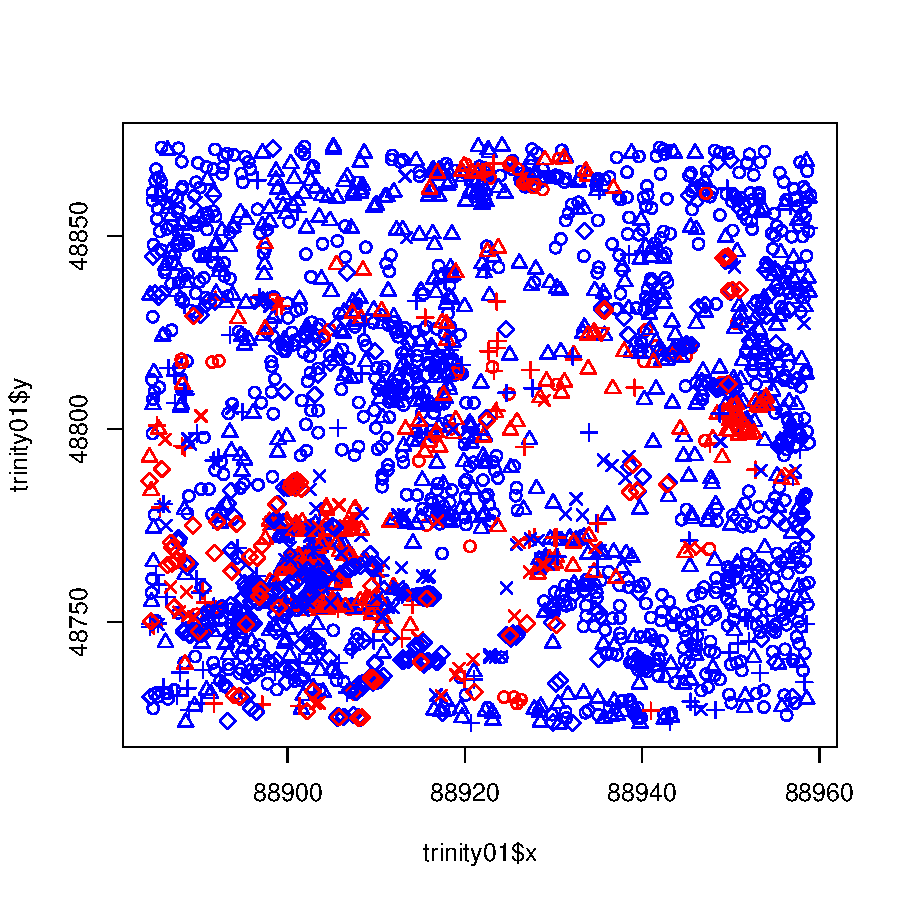
\includegraphics{disperseRmanual-009}


And now let's establish the seedling subplots, and get a list of seedlings within:

\begin{Schunk}
\begin{Sinput}
> trinSubplotPoints <- getBufferedPoints(x=trinity01$x,
+                   y=trinity01$y,
+                   buffer=0,
+                   systematic=TRUE,
+                   by=1)
> trinSeedlingDensity <- sampleSubplots(trinSubplotPoints,
+                                       trinity01,
+                                       subplotsize=1)
> nrow(trinSeedlingDensity)
\end{Sinput}
\begin{Soutput}
[1] 8
\end{Soutput}
\end{Schunk}


\begin{Schunk}
\begin{Sinput}
> formula <- "numseedlings~(dbh/30)^2 * exp(-m^3)"
\end{Sinput}
\end{Schunk}

We will do the normalizer afterwards, because it should not affect the outcome of the model. Now that we have the data.frame and the model, it's a simple matter of running it. Because it is nonlinear, we need to use nls() with some start values.


\bibliographystyle{sty/ecology}
\bibliography{disperseRmanual}
\end{document}
